
\section{Perspectives of the IDS-RAM}
Directly related to the five layers of the IDS-RAM are three cross-sectional perspectives: \textit{Security}, \textit{Certification}, and \textit{Governance}. These are described in detail in the following sections.

\subsection{Security Perspective}
%\addcontentsline{toc}{subsection}{Security Perspective}
As stated in Section 1.1, one strategic requirement of the International Data Spaces is to provide secure data supply chains. This is critical for establishing and maintaining trust among Participants that want to exchange and share data and use Data Apps. The IDS Security Architecture provides means to identify Participants,, protect communication and data exchange transactions, and control the use of data after it has been exchanged.

For these purposes, the International Data Spaces defines a Trusted Connector as an extension of the Base Connector (see Section 3.5). The IDS Connector ensures that the specifications and requirements of the Security Architecture materialize in everyday interactions and operations in the International Data Spaces. The security aspects described in the following constitute the basis of the IDS Connector. The differences between a Trusted Connecter and a Base Connector are detailed in the Security Profiles subsection 4.1.3.3.6.

\subsubsection{Security Aspects Addressed by the Different Layers of the IDS-RAM}
%\addcontentsline{toc}{subsubsection}{Security Aspects Addressed by the Different Layers of the IDS-RAM}

\paragraph*{Business Layer\\}

Security aspects are crucial for the definition of roles and basic interaction patterns in the International Data Spaces.

\paragraph*{Functional Layer\\}

Security requirements may restrict certain transactions or operations in the International Data Spaces, or even prevent them. However, security is also an enabling factor. Without security, many use cases would not be possible (e.g., offering sensitive data to trusted business partners). The concept of data usage control allows Data Providers to attach data usage policy information to their data in order to define how a Data Consumer may use the data.

\paragraph*{Process Layer\\}

To take security aspects into account on the Process Layer, it is important that existing processes are permanently monitored, validated, and redesigned, if need be. For example, to allow trustworthy identification and authentication of Participants using a central public key infrastructure (PKI), a Participant must apply for a public key certificate that is registered in a central PKI and deployed inside its Connector. For dynamic attribute support, an identity management server needs to verify attributes before issuing access tokens. The same is true for trustworthy operations of an App Store, for which data must be verified and signed by a trusted entity before it can be uploaded.

\paragraph*{Information Layer\\}

The Information Layer provides the means for Participants to use a common vocabulary and common semantics to express concepts and relationships between them. In doing so, it is possible to specify access and usage control policies in a way that these are understood by all Participants. The same is true for access control requirements defining minimum security profiles, which must be met before access is granted.

\paragraph*{System Layer\\}

As the Connector is the central technical component on the System Layer, it is predominantly the Connector where the security features of the International Data Spaces are implemented. Being an extension of the Base Connector, the Trusted Connector takes up all relevant security specifications and requirements, and serves as the technological basis for use case implementations.

\subsubsection{General Security Principles}
%\addcontentsline{toc}{subsubsection}{General Security Principles}
The development of the Security Architecture follows two general principles:

\paragraph*{Use of existing standards and consideration of best practices\\}

To the extent possible and reasonable, existing standards and best practices are to be used and leveraged in the development of the Security Architecture. The aim of the Security Architecture is not to offer new solutions for problems already solved, but to combine existing, reliable approaches in a useful and meaningful way, and bridge gaps where necessary.

\paragraph*{Scalability of security levels\\}

The International Data Spaces does not enforce a single level of security to be applied for all Participants. This way, also organizations with limited resources and technical means are able to participate (at least as Data Consumers). However, also the security level of these participants must be reliable and verifiable for others. Certain minimum security requirements (e.g., encrypted communication) therefore need to be met by all Participants.

Provided a Participant is in line with general security requirements, it may decide about the level of security to be applied for it itself. It should be noticed, however, that data sources may presuppose a certain minimum level of security to be met by potential Data Consumers. This means for Data Consumers: the higher the security level they choose for themselves to be applied, the better the access to high-quality data sources and high-value data services.

\subsubsection{Key Security Concepts}
%\addcontentsline{toc}{subsubsection}{Key Security Concepts}
The Security Architecture addresses seven key security concepts: 1) secure communication, 2) identity management, 3) trust management, 4) trusted platform, 5) data access control, 6) data usage control and 7) data provenance tracking. 

\paragraph{Secure Communication\\}
%\addcontentsline{toc}{paragraph}{Secure Communication}
To ensure confidentiality and authenticity of data transfers, communication between Connectors must be protected. When using the IDS Connector, two layers of security are in place:

\begin{itemize}
	\item point-to-point encryption (between Connectors), using an encrypted tunnel, and

	\item end-to-end authorization (authenticity and authorization based on actual communication endpoints; i.e., Data Apps).
\end{itemize}

Data from one External Connector to another is sent over the Internet or via a virtual private network (VPN), the specification of which is beyond the scope of the IDS Security Architecture. The Security Architecture defines the IDS Communication Protocol (IDSCP), which must be supported by Trusted Connectors, and can be supported by any other Connector as well. The purpose of the IDSCP is to establish confidential, authenticated communication, exchange data between the Data Provider and the Data Consumer, and establish mutual remote attestation (if supported by the Connectors involved). IDS Connectors must communicate with each other over an encrypted tunnel (e.g., TLS), as depicted in Figure 41, and may use IDSCP or another appropriate protocol, like https or mqtt.



%%%%%%%%%%%%%%%%%%%% Figure/Image No: 42 starts here %%%%%%%%%%%%%%%%%%%%

\begin{figure}[H]
	\begin{Center}
		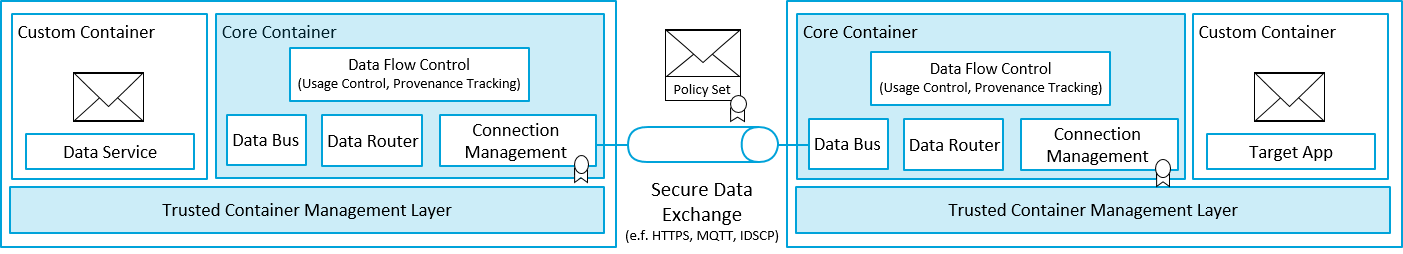
\includegraphics[width=6.53in,height=1.18in]{./media/image57.png}
		\caption{ IDS Communication }
		\label{fig:_IDS_Communication_}
	\end{Center}
\end{figure}


%%%%%%%%%%%%%%%%%%%% Figure/Image No: 42 Ends here %%%%%%%%%%%%%%%%%%%%


The IDSCP is a high-level protocol established via WebSocket Secure (WSS). It contains several $``$conversations$"$ , which can be initiated by either side and must be confirmed by the other side to be entered. Currently, two conversations are provided: remote attestation and metadata exchange. The protocol itself is performed inside a tunneled connection.

The protocol supports and enables several communication aspects:

\begin{itemize}
	\item identification and authentication,

	\item remote attestation,

	\item metadata exchange, and

	\item data exchange (together with usage policy information attached).

\end{itemize}

The last aspect, data exchange, provides the basic mechanism of data usage control, as it is possible to attach data usage policy information in order to specify how the data may be used by the Data Consumer. However, the specification of the IDSCP is not part of this document.

\paragraph{Identity Management\\}
%\addcontentsline{toc}{paragraph}{Identity Management}
To be able to make access control related decisions that are based on reliable identities and properties of Participants, a concept for Identity and Access Management (IAM) is mandatory. The following aspects are central for the concept:

\begin{itemize}
	\item identification (i.e., claiming an identity),

	\item authentication (i.e., verifying an identity), and

	\item authorization (i.e., making access decisions based on an identity).
\end{itemize}

The \textit{Certificate} \textit{Authority (CA)} issues certificates for all entities. These certificates are used for authentication and encryption between Connectors.

An identity may have several attributes, which are linked to that identity. A Dynamic Attribute Provisioning Service (DAPS) is used to provide dynamic, up-to-date attribute information about Participants and Connectors.

\subparagraph*{Mapping of Participant Certification and Connector Certification to Identity Management\\}
%\addcontentsline{toc}{subparagraph}{Mapping of Participant Certification and Connector Certification to Identity Management}
There are two targets of certification: Participants (receiving a Participant Certificate) and Core Components (receiving a Core Component Certificate). If a Participant (e.g., a company) is successfully certified, it is allowed to participate in the International Data Spaces. The Participant has to use a certified IDS Connector. With both certificates, the Participant Certificate and the Core Component Certificate, the Participant can request a digital X.509 certificate for identification, authentication, and encryption.

A X.509 certificate contains only the most relevant, static information:

\begin{itemize}
	\item \textbf{C (countryName):} country of the organization (e.g. DE);

	\item \textbf{O (organizationName):} name of the organization (e.g. Fraunhofer); 

	\item \textbf{OU (organizationalUnitName):} name of the organizational unit (e.g. AISEC),

	\item \textbf{CN (commonName):} Universally Unique Identifier (UUID) (e.g. 59C3BAE6-1C06-4723-802B-12C7DCF94E58);


	\item \textbf{subjectAltName (X509v3 Subject Alternative Name):} is filled with DNS entries / IP addresses of the Connector ( e.g.\\
DNS.1 = localhost\\
DNS.2 = idsconnector.aisec.fraunhofer.de\\
IP.1 = 0.0.0.0\\
IP.2 = 10.1.2.15\\
IP.3 = 10.1.2.16\\
IP.4 = 10.1.2.17\\
IP.5 = 10.1.2.18\\
)
\end{itemize}


It is important to note that any modification of attributes leads to revocation and reissuing of the certificate. For this reason, the number of attributes that are contained in a certificate needs to be kept at a minimum. Dynamic attributes are kept by the Dynamic Attribute Provisioning Service (DAPS).

\subparagraph*{Proposed PKI Structure\\}
%\addcontentsline{toc}{subparagraph}{Proposed PKI Structure}
In general, a PKI can have several layers to achieve separation of duties (i.e., every Sub-CA is responsible for a specific topic). Depending on the business and deployment model applied, several Sub-CAs may exist.



%%%%%%%%%%%%%%%%%%%% Figure/Image No: 43 starts here %%%%%%%%%%%%%%%%%%%%

\begin{figure}[H]
	\begin{Center}
		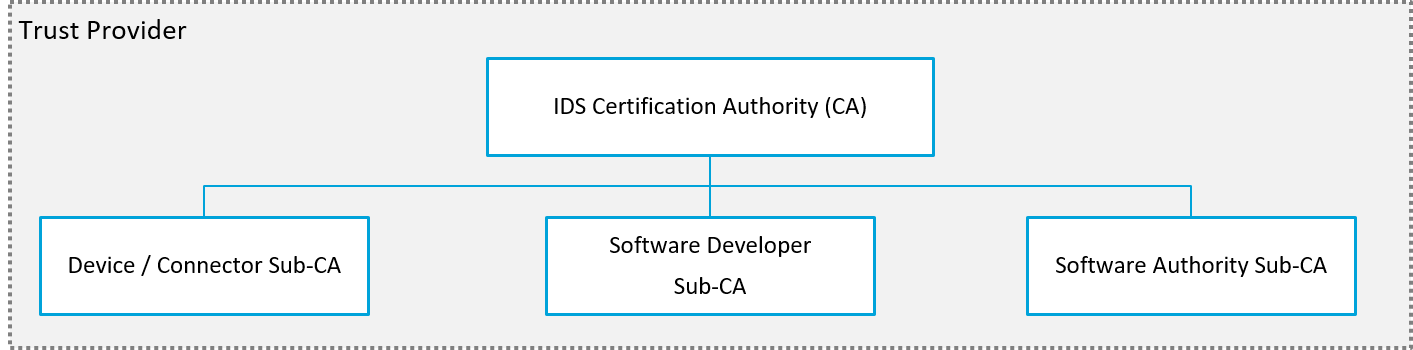
\includegraphics[width=6.53in,height=1.62in]{./media/image58.png}
		\caption{ PKI structure (example)}
		\label{fig:_PKI_structure_example}
	\end{Center}
\end{figure}


%%%%%%%%%%%%%%%%%%%% Figure/Image No: 43 Ends here %%%%%%%%%%%%%%%%%%%%


This allows for specific parties to issue certificates for specific purposes. It is also possible to support multiple instances (e.g., multiple Connector Sub-CAs). The structure of the PKI is not defined in this document.

\subparagraph*{Connector Certificate Deployment\\}
%\addcontentsline{toc}{subparagraph}{Connector Certificate Deployment}
After obtaining the Participant Certificate and a Core Component Certificate, an organization may apply for one or more X.509 Certificates (the issuing of which may be triggered by the International Data Spaces Association, for example).

The attributes for Connectors to be embedded in the X.509 certificate are defined above.

Once received, the Connector Certificate can be deployed onto the Connector.



%%%%%%%%%%%%%%%%%%%% Figure/Image No: 44 starts here %%%%%%%%%%%%%%%%%%%%

\begin{figure}[H]
	\begin{Center}
		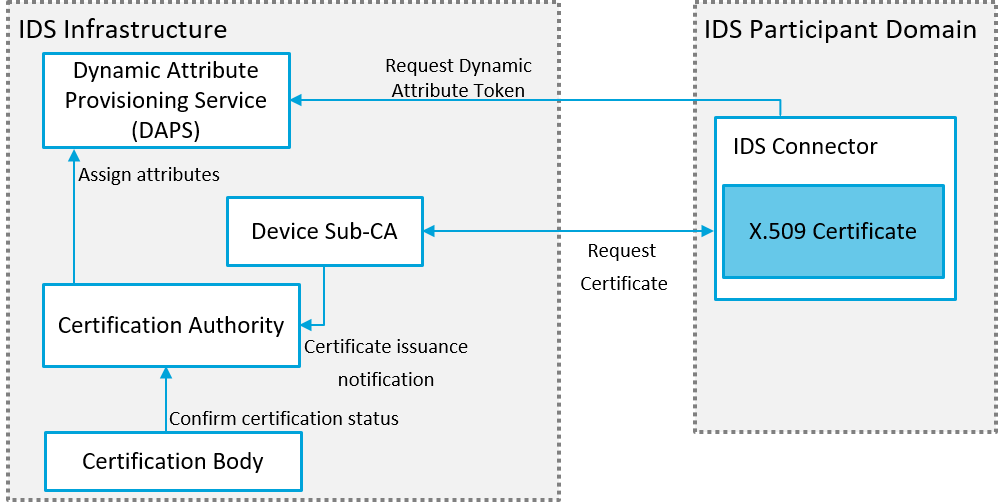
\includegraphics[width=6.53in,height=3.29in]{./media/image59.png}
		\caption{ Embedding the Connector Certificate }
		\label{fig:_Embedding_the_Connector_Certificate_}
	\end{Center}
\end{figure}


%%%%%%%%%%%%%%%%%%%% Figure/Image No: 44 Ends here %%%%%%%%%%%%%%%%%%%%


The X.509 Certificate ensures that data is always exchanged in an authenticated and encrypted manner.

\subparagraph*{Using the Dynamic Attribute Provisioning Service (DAPS) for Identity Management \\}
%\addcontentsline{toc}{subparagraph}{Using the Dynamic Attribute Provisioning Service (DAPS) for Identity Management }
Using a service to hand out attributes in a dynamic fashion reduces the need for certificate revocation and enables more flexible attribute handling for participants in the International Data Spaces. This allows dynamic assignment of attributes and status flags to Connector instances. Examples of status flags are:

\begin{itemize}
	\item Withdraw a security status if known vulnerabilities have not been fixed.

	\item Upgrade the certification status without reissuing a X.509 certificate.

	\item Assign membership status to a workflow with contractors.

	\item Notification of temporary changes of a Participant’s level of trustworthiness.

	\item Provisioning of mutable attributes (e.g. address of the organization).

\end{itemize}

This concept avoids revocation of certificates in most cases, as it allows to include new attributes if need arises.

\subparagraph*{Using an Authorization Service for Resource Access Control \\}
%\addcontentsline{toc}{subparagraph}{Using an Authorization Service for Resource Access Control}
Using an Authorization Service (featuring access tokens) allows use case dependent modeling of access control decisions. Delegation of access decisions is possible. In complex workflows, multiple Connectors can use a dedicated Authorization Service to delegate resource access decisions. The DAPS acts as the Authorization Service for the IDS.



%%%%%%%%%%%%%%%%%%%% Figure/Image No: 45 starts here %%%%%%%%%%%%%%%%%%%%

\begin{figure}[H]
	\begin{Center}
		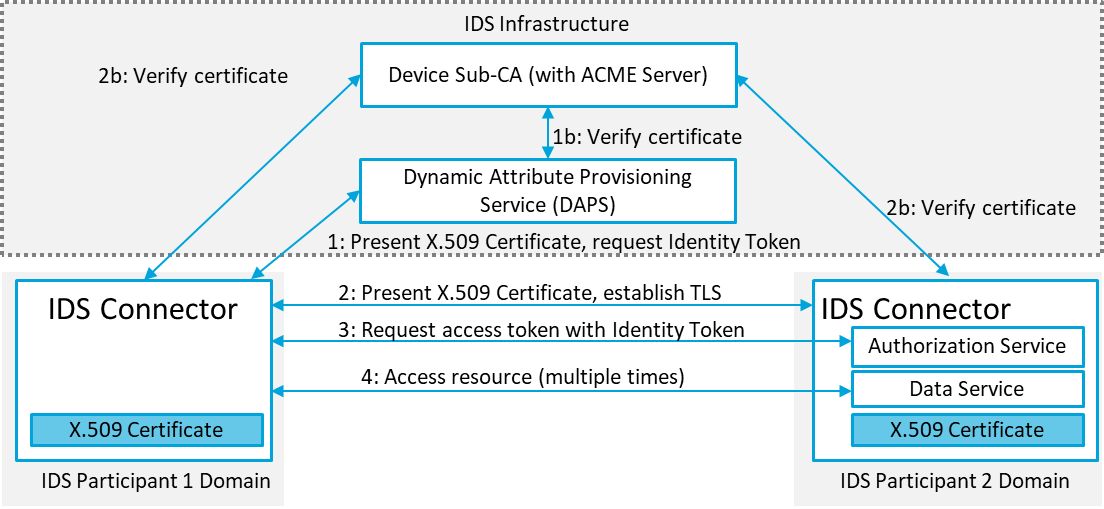
\includegraphics[width=7.36in,height=3.39in]{./media/image60.png}
		\caption{ Resource access workflow}
		\label{fig:_Resource_access_workflow}
	\end{Center}
\end{figure}


%%%%%%%%%%%%%%%%%%%% Figure/Image No: 45 Ends here %%%%%%%%%%%%%%%%%%%%


A workflow for accessing a resource (e.g., a Data Service) using dynamic attributes and access tokens is defined as follows:

\begin{enumerate}[label*=\arabic*.]
	\item A Dynamic Attribute Token (DAT) is requested from the Dynamic Attribute Provisioning Service, presenting the Connector's X.509 certificate. Depending on the verification policy specified, the attribute can be verified at the CA.

	\item Before accessing a resource, a TLS tunnel is established using the same X.509 certificate. Again, depending on the policy specified, the certificate can be verified at the CA.

	\item (Optional) If using several Access Tokens (ATs), a token request is performed at a separate Authorization Service in the domain of a use case operator or the domain of the Connector's (or, more specifically, resource’s) owner.

	\item The resource is requested by handing in either the Dynamic Attribute Token (DAT) or the Access Token (AT).
\end{enumerate}

Due to the small size of access tokens, it is possible to incorporate these tokens into any resource request and support stateless access management. Both DATs and ATs use the JSON Web Token (IETF RFC 7519)\footnote{ https://tools.ietf.org/html/rfc7519 } standard.

\paragraph*{Trust Management \\}
%\addcontentsline{toc}{paragraph}{Trust Management}
To establish trust across the entire business ecosystem (i.e., to protect Participants from fraud and ensure they abide by the designated rules), the International Data Spaces makes use of cryptographic methods. One such method is the public key infrastructure (PKI). A central principle of a PKI is that every entity is allocated with secret keys, allowing each entity to authenticate against other Participants. Thereby, a hierarchy is created, with the Identity Provider on top issuing certificates to the other entities, which in turn may issue certificates to other entities, and so on. In the following, the PKI rollout is described for mapping roles and entities required for the deployment of the International Data Spaces.



%%%%%%%%%%%%%%%%%%%% Figure/Image No: 46 starts here %%%%%%%%%%%%%%%%%%%%

\begin{figure}[H]
	\begin{Center}
		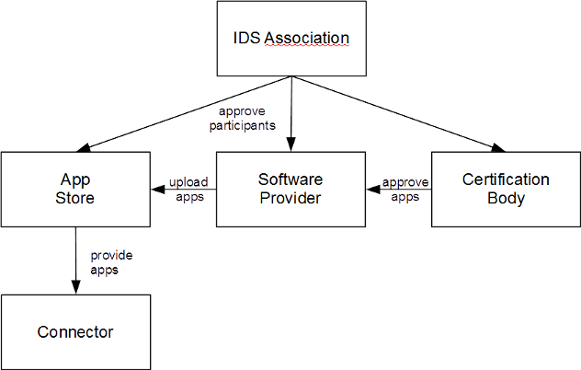
\includegraphics[width=4.85in,height=3.09in]{./media/image61.png}
		\caption{ Technical roles in the International Data Spaces}
		\label{fig:_Technical_roles_in_the_International_Data_Spaces}
	\end{Center}
\end{figure}


%%%%%%%%%%%%%%%%%%%% Figure/Image No: 46 Ends here %%%%%%%%%%%%%%%%%%%%


\subparagraph*{PKI Rollout\\}
%\addcontentsline{toc}{subparagraph}{PKI Rollout}
To guarantee secure identity management, the International Data Spaces defines technical roles for implementing a PKI system that is flexible enough to support all roles defined on the Business Layer. In particular, six entities with different security levels are relevant for the Security Architecture. In the following, these entities and the technical roles related to them are described. 

\subparagraph*{Identity Provider\\}

The Identity Provider acts as an agent for the International Data Spaces Association. It is responsible for issuing technical identities to parties that have been approved to become Participants in the International Data Spaces. The Identity Provider is instructed to issue identities based on approved roles (e.g., App Store or App Provider). Only if equipped with such an identity, an entity is allowed to participate in the International Data Spaces (e.g., to provide data or publish Data Apps). The Identity Provider may exclude Participants from the International Data Spaces, if instructed to do so. 

As a trusted entity, the Identity Provider manages the PKI rollout. It takes care if certificates expire or must be revoked. There are two separate PKI hierarchies: one for software signatures (Software Signing Root CA) and one for the Connectors (Service Root CA). An entity is assigned with either an end certificate or a sub/root-CA certificate. The two hierarchies protect the interests of the six entities.



%%%%%%%%%%%%%%%%%%%% Figure/Image No: 47 starts here %%%%%%%%%%%%%%%%%%%%

\begin{figure}[H]
	\begin{Center}
		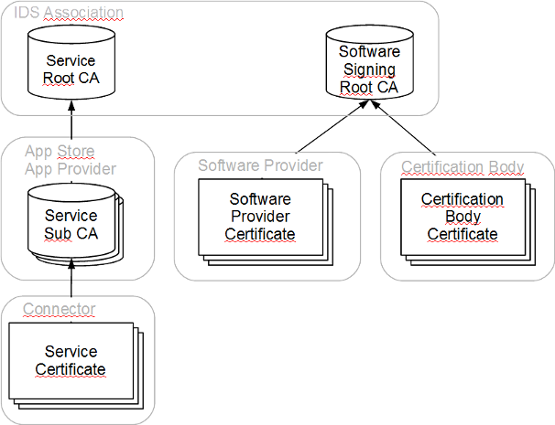
\includegraphics[width=4.63in,height=3.55in]{./media/image62.png}
		\caption{ Mapping of technical roles and PKI layout}
		\label{fig:_Mapping_of_technical_roles_and_PKI_layout}
	\end{Center}
\end{figure}


%%%%%%%%%%%%%%%%%%%% Figure/Image No: 47 Ends here %%%%%%%%%%%%%%%%%%%%


\subparagraph*{Software Provider \\}

A Software Provider produces and distributes basic software stacks for Connectors (for rollout and deployment). To every Software Provider seeking admission to the International Data Spaces, the Identity Provider issues a service sub-CA request. An approved Software Provider uses the service sub-CA during rollout and deployment of the Connector in order to provide it with an initial, valid and preconfigured system.

\subparagraph*{Connector \\}

A Connector is allowed to communicate with other Connectors only if acquired from an approved Software Provider. Connectors download Data Apps from the App Store. For each Data App downloaded, the Connector creates a service key pair and a Certificate Signing Request (CSR). While the private key is used to identify the Data App and to protect its data, the CSR is sent to the App Store, which uses it to issue a certificate. This also allows entities to check whether the license of a certain Data App is still valid (see e.g. remote attestation). Furthermore, the private key and the certificate are used for establishing a secure channel with other Connectors. During rollout, the Software Provider deploys an initial system onto the Connector and signs the Connector's corresponding service CSRs for the initial system.

\subparagraph*{App Store \\}

A Connector downloads the software it requires (i.e. Data Apps) from an App Store. Connectors can only connect with the App Store for requesting downloads and updates. As the App Store is a Connector itself, it additionally stores its own sub-CA. When a new provider sets up an App Store, the Identity Provider signs a sub-CA request issued by the App Store provider. The App Store provider deploys this sub-CA inside the App Store (i.e., inside the respective Connector). This sub- CA is used by the App Store to ensure the validity of services downloaded by other Connectors. This means that if an App Store signs a CSR (i.e., issues a certificate), a Connector receives a certificate for a downloaded Data App.

\subparagraph*{App Provider \\}

App Providers must seek approval of Data Apps from the Certification Body. Upon successful certification of a Data App, the App Provider may publish the Data App by uploading it to the App Store. Each App Provider can be unambiguously identified by a certificate issued by the Identity Provider.

\subparagraph*{Certification Body \\}

When an App Provider uploads a Data App, the App Store not only checks if the Data App comes from an approved App Provider, but also if the software meets certain quality and security standards. Therefore, App Providers must send the Data App to a Certification Body for inspection. The Certification Body checks the validity of the App Provider’s signature. If the signature is valid, the source code of the respective Data App is inspected. If the Data App meets the quality and security standards, the Certification Body signs the Data App with the certificate's private key. To do so, it does not need a sub-CA, as it only signs the software, but does not create a certificate.

\subparagraph*{Connector Manifestations \\}
%\addcontentsline{toc}{subparagraph}{Connector Manifestations}
A Connector can run different services and communicate with other Connectors. Using the PKI, a Connector protects the persistent storage of its services and the communication with other Connectors (in terms of authenticity, confidentiality, etc.). The following items characterize a Connector in the International Data Spaces from the security perspective:

\subparagraph*{Configuration \\}

Among other things, the configuration specifies from where the Connector downloads new services, or which Brokers or Online Certificate Status Protocol (OCSP)\footnote{ https://tools.ietf.org/html/rfc6960 } servers it uses. Configuration is required in order to boot the system. It is executed during the Connector’s deployment.

\subparagraph*{CA Certificates \\}

In order to verify PKI signatures (e.g., for authentication or for Data Apps that were downloaded), the Connector stores the trusted root certificates (Service Root CA and Software Signing Root CA) in a way their integrity is preserved (Figure 47).

\subparagraph*{Apps \\}
%\addcontentsline{toc}{subparagraph}{Apps}
Apps offered in the International Data Spaces run inside isolated containers (see section 3.5.1.2 for details). The Connector creates a key pair for every App it downloads. The private key protects the App’s persistent data. When downloading an App from the App Store, the Connector creates a CSR using the public key. The App Store signs the CSR and issues a certificate. The Connector uses this certificate to make sure that the App it is running is valid (i.e., licensed, not expired, etc.).

An App is a generalization of the following types of software:

\begin{itemize}
	\item \textit{Core System}: Every Connector runs exactly one Core System. The Core System, together with its certificate, is deployed during the Connector’s deployment after being retrieved from the Software Provider providing the Connector. The Core System’s certificate identifies the underlying hardware device. The Core System can connect to other Connectors (e.g., to communicate with the App Store for app downloads). When a Connector establishes a communication channel with another Connector, it uses the Core System’s private key and certificate for authentication.

	\item \textit{Data App:} A Data App is any data processing or data collecting app, or a System Adapter.

	\item \textit{Broker:} A Broker is a Connector providing a broker service.

	\item \textit{OCSP Server}: A Connector is considered an OCSP Server if it runs the OCSP Server app.

	\item \textit{App Store:} An App Store has a service sub CA. The International Data Spaces Association signs this CSR in order to approve every new App Store. The CSR identifies the App Store and makes it possible to sign the service CSRs from the Connectors requesting apps.

\end{itemize}



%%%%%%%%%%%%%%%%%%%% Figure/Image No: 48 starts here %%%%%%%%%%%%%%%%%%%%

\begin{figure}[H]
	\begin{Center}
		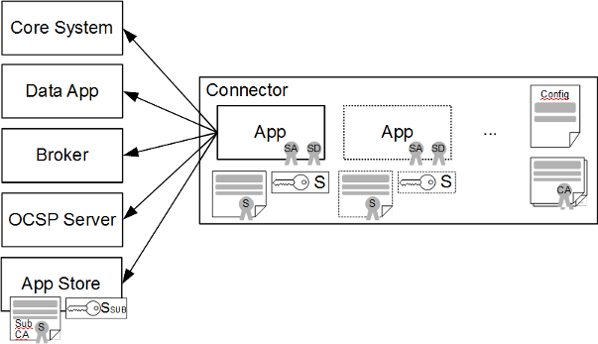
\includegraphics[width=4.98in,height=2.86in]{./media/image63.png}
		\caption{e Identity Provider also acts as an authorization service (as described above) by incorporating the DAPS.}
		\label{fig:e_Identity_Provider_also_acts_as_an_authorization_service_as_described_above_by_incorporating_the_DAPS}
	\end{Center}
\end{figure}


%%%%%%%%%%%%%%%%%%%% Figure/Image No: 48 Ends here %%%%%%%%%%%%%%%%%%%%

\subparagraph*{App Development and Deployment \\}
%\addcontentsline{toc}{subparagraph}{App Development and Deployment}
The following steps describe the lifecycle of Data Apps used in the International Data Spaces, from an app’s development to its deployment onto a Connector (Figure 48):

\begin{enumerate}[label*=\arabic*.]
	\item The Identity Provider signs a key pair and a certificate for each Software Provider on behalf of the International Data Spaces Association. When the app is fully developed and ready for being offered, the Software Provider signs the app using its private key, before the signed app is sent to a trusted Certification Body.

	\item If the Certification Body approves the app, a second signature is added to it.

	\item The Software Provider uploads the app to an App Store; the app thereby becomes an IDS Data App. The App Store only accepts valid (i.e., correctly signed) Data Apps (since the App Store is a Connector with corresponding root CAs, it is able to verify all signatures).

	\item A Connector downloading the Data App connects with the App Store. The Connector creates a service key pair and a CSR, requests a service download, and sends the CSR to the App Store. The App Store signs the CSR using the service sub-CA and returns it to the Connector.

	\item The Connector downloads the service and checks its signatures. If the signatures are found to be valid, the Connector installs the service. From now on, the downloading Connector can check the validity of the downloaded service based on the certificate received.
\end{enumerate}



%%%%%%%%%%%%%%%%%%%% Figure/Image No: 49 starts here %%%%%%%%%%%%%%%%%%%%

\begin{figure}[H]
	\begin{Center}
		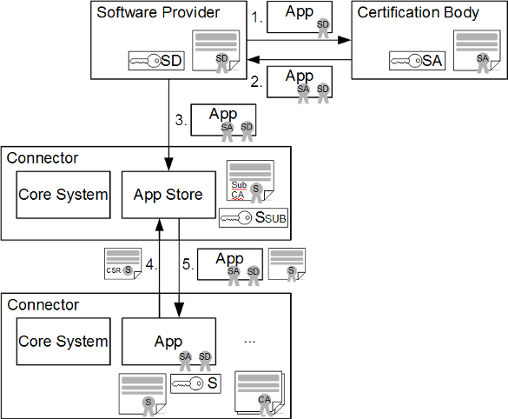
\includegraphics[width=4.24in,height=3.48in]{./media/image64.png}
		\caption{Software development, approval, and download process}
		\label{fig:Software_development_approval_and_download_process}
	\end{Center}
\end{figure}


%%%%%%%%%%%%%%%%%%%% Figure/Image No: 49 Ends here %%%%%%%%%%%%%%%%%%%%

\subparagraph*{Delivery of Connectors \\}
%\addcontentsline{toc}{subparagraph}{Delivery of Connectors}
After initial deployment, the Connector is delivered to the Operator in a fully preconfigured state (Figure 49). For deployment of the Connector, every approved Software Provider has a sub-CA key pair and CSR (similar to an App Store Provider) to sign the initial system. When the Identity Provider signs the CSR of the sub-CA, it confirms the requesting Software Provider as being compliant with International Data Spaces regulations and policies. The Operator of a Connector (e.g., a Data Provider) can change the configuration, the root certificates, and even the Core System as deemed appropriate.



%%%%%%%%%%%%%%%%%%%% Figure/Image No: 50 starts here %%%%%%%%%%%%%%%%%%%%

\begin{figure}[H]
	\begin{Center}
		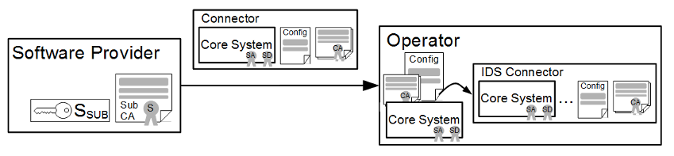
\includegraphics[width=5.17in,height=1.2in]{./media/image65.png}
		\caption{ Delivery of a Connector}
		\label{fig:_Delivery_of_a_Connector}
	\end{Center}
\end{figure}


%%%%%%%%%%%%%%%%%%%% Figure/Image No: 50 Ends here %%%%%%%%%%%%%%%%%%%%


\subparagraph*{Connector Security Profiles \\}
%\addcontentsline{toc}{subparagraph}{Connector Security Profiles}

Static security levels would make it necessary to anticipate all possible needs of every Participant, now and in the future. Since the IDS is designed to grow over time, and remain flexible with regard to the individual security needs of every participant, it offers the possibility to base access control decisions on fully customized criteria. Access control policies can be based on a set of attributes of the requesting Connector. Besides a unique identifier, these attributes include a set of properties describing the security level of Data Apps as well as the security properties of the technical setup of the Connector and the organizational capabilities of the Participant. A set of security properties is called a Security Profile.



A Security Profile comprises attributes of the Connector and may be used in an attribute-based access control policy. Each Connector must provide its Security Profile upon request. The Security Profile must never be empty.


A Security Profile contains the following properties:
\begin{itemize}
\item  It describes the Connector’s current security configuration.
\item  It allows Data Consumers to decide whether they are willing to rely on data provided by a Data Provider's endpoint.
\item  It allows Data Providers to decide whether they are willing to make sensitive data available to a Data Consumer.
\end{itemize}

The IDS-RAM defines four different Security Profiles: Base Free, Base, Trust, and Trust+ (Managed Trust):

\begin{itemize}
	\item The $``$Base Free$"$  Security Profile allows using IDS concepts and technologies outside the trusted business ecosystem (e.g. for research projects or for operation within a particular security domain like an internal company network). 

	\item The $``$Base$"$  Security Profile defines the mechanisms required for a minimum level of trust, including the certification process. 

	\item The $``$Trust$"$  Security Profile allows definition of extended security features.

	\item The $``$Trust+$"$  (Managed Trust) Security Profile relies on trusted hardware based on TPM. 
\end{itemize}

More profiles may be added in the future.

To define a $``$common sense$"$  for every IDS Participant and Connector, and to distinguish the different Security Profiles, four dimensions are defined:


\begin{itemize}
	\item Development, relating to the requirements and capabilities regarding the development of components;

	\item IDS Roles supported, relating to the IDS Roles (as described in section 3.1) supported by the respective Security Profile;

	\item Communication abilities supported, specifying the communication features supported by the respective Security Profile; and

	\item Higher security features, specifying the security level provided by the respective Security Profile. 
\end{itemize}




%%%%%%%%%%%%%%%%%%%% Table No: 9 starts here %%%%%%%%%%%%%%%%%%%%


\begin{table}[H]
 			\centering
\begin{tabular}{p{0.76in}p{1.18in}p{0.98in}p{1.08in}p{1.37in}}
\hline
%row no:1
\multicolumn{1}{|p{0.76in}}{} & 
\multicolumn{1}{|p{1.18in}}{{\fontsize{8pt}{9.6pt}\selectfont \textbf{Base Free}}} & 
\multicolumn{1}{|p{0.98in}}{{\fontsize{8pt}{9.6pt}\selectfont \textbf{Base}}} & 
\multicolumn{1}{|p{1.08in}}{{\fontsize{8pt}{9.6pt}\selectfont \textbf{Trust}}} & 
\multicolumn{1}{|p{1.37in}|}{{\fontsize{8pt}{9.6pt}\selectfont \textbf{Trust+}}} \\
\hhline{-----}
%row no:2
\multicolumn{1}{|p{0.76in}}{{\fontsize{8pt}{9.6pt}\selectfont \textbf{Development }}} & 
\multicolumn{1}{|p{1.18in}}{{\fontsize{8pt}{9.6pt}\selectfont Developed as Open Source}} & 
\multicolumn{1}{|p{0.98in}}{{\fontsize{8pt}{9.6pt}\selectfont Developed in the IDSA Community}} & 
\multicolumn{1}{|p{1.08in}}{{\fontsize{8pt}{9.6pt}\selectfont Developed in the IDSA Community}} & 
\multicolumn{1}{|p{1.37in}|}{{\fontsize{8pt}{9.6pt}\selectfont Developed in the IDSA Community and bound to strong SLA regarding security updates.}} \\
\hhline{-----}
%row no:3
\multicolumn{1}{|p{0.76in}}{{\fontsize{8pt}{9.6pt}\selectfont \textbf{IDS Roles supported}}} & 
\multicolumn{1}{|p{1.18in}}{{\fontsize{8pt}{9.6pt}\selectfont Not certified, therefore the public IDS infrastructure is not available}} & 
\multicolumn{1}{|p{0.98in}}{{\fontsize{8pt}{9.6pt}\selectfont All IDS Roles (section 3.1.1) supported, but support for Clearing House is optional}} & 
\multicolumn{1}{|p{1.08in}}{{\fontsize{8pt}{9.6pt}\selectfont All IDS Roles (section 3.1.1) supported,}} & 
\multicolumn{1}{|p{1.37in}|}{{\fontsize{8pt}{9.6pt}\selectfont All IDS Roles (section 3.1.1) supported,}} \\
\hhline{-----}
%row no:4
\multicolumn{1}{|p{0.76in}}{{\fontsize{8pt}{9.6pt}\selectfont \textbf{Communication abilities supported}}} & 
\multicolumn{1}{|p{1.18in}}{{\fontsize{8pt}{9.6pt}\selectfont Cannot connect to public IDS services or connectors.}} & 
\multicolumn{1}{|p{0.98in}}{{\fontsize{8pt}{9.6pt}\selectfont Can connect to other connectors and exchange data.}} & 
\multicolumn{1}{|p{1.08in}}{{\fontsize{8pt}{9.6pt}\selectfont Can connect to other connectors and exchange data. Can refuse a connection with a Connector with Base Profile.}} & 
\multicolumn{1}{|p{1.37in}|}{{\fontsize{8pt}{9.6pt}\selectfont Can connect to other connectors and exchange data. Can refuse a connection with a Connector with Base Profile.}} \\
\hhline{-----}
%row no:5
\multicolumn{1}{|p{0.76in}}{{\fontsize{8pt}{9.6pt}\selectfont \textbf{Higher security features }}} & 
\multicolumn{1}{|p{1.18in}}{{\fontsize{8pt}{9.6pt}\selectfont Security level not defined }} & 
\multicolumn{1}{|p{0.98in}}{{\fontsize{8pt}{9.6pt}\selectfont Standard security level }} & 
\multicolumn{1}{|p{1.08in}}{{\fontsize{8pt}{9.6pt}\selectfont Extended security level }} & 
\multicolumn{1}{|p{1.37in}|}{{\fontsize{8pt}{9.6pt}\selectfont High security level}} \\
\hhline{-----}

\end{tabular}
 \end{table}


%%%%%%%%%%%%%%%%%%%% Table No: 9 ends here %%%%%%%%%%%%%%%%%%%%


The attributes of the Security Profiles are listed in Appendix B of this document. 

\paragraph{Trusted Platform \\}
%\addcontentsline{toc}{paragraph}{Trusted Platform}
The International Data Spaces consists of multiple manifestations of the Connector Architecture (as used by e.g. the Broker or the App Store). This is why a trusted platform is a central element of trustworthy data exchange. A trusted platform comprises certain key aspects:

\begin{itemize}
	\item To be able to specify minimal requirements for Participants that want to exchange data, a common understanding of each other’s Security Profiles needs to be established. The Connector supports mutual verification of these profiles.

	\item To enable trustworthy execution of Data Apps and guarantee system integrity, strong isolation of components is necessary. The Connector's application container management supports full isolation of Data Apps deployed, and limitation of illegitimate communication channels. This means that Data Apps have access only to data that is explicitly meant for them.

	\item To establish a trustworthy relationship with another Participant, and to verify Connector properties, remote integrity verification is required. The Connector features a hardware-based trust anchor and a trustworthy software stack.
\end{itemize}

\subparagraph*{Isolation and Remote Execution Guarantee \\}
%\addcontentsline{toc}{subparagraph}{Isolation and Remote Execution Guarantee}
Isolation is a form of integrity enforcement for a Data App’s runtime environment. Data Apps can be isolated against each other by deploying each one inside a separate container (or all Data Apps of a specific Software Provider into one container), as illustrated in Figure 410. This allows implementation of additional security features, such as time-to-live policy enforcement for complete container instantiations.



%%%%%%%%%%%%%%%%%%%% Figure/Image No: 51 starts here %%%%%%%%%%%%%%%%%%%%

\begin{figure}[H]
	\begin{Center}
		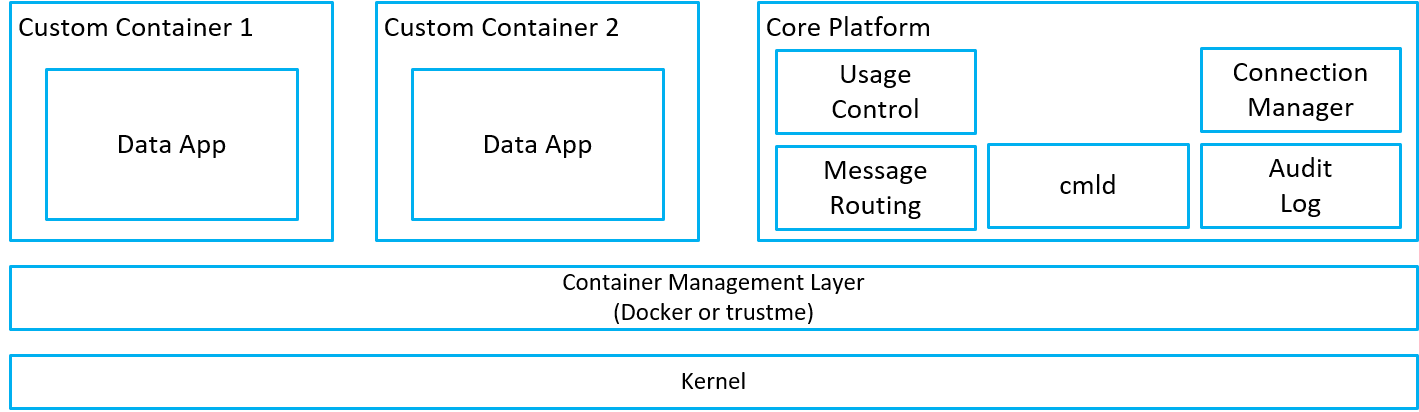
\includegraphics[width=6.4in,height=2.02in]{./media/image66.png}
		\caption{Container isolation for Data Apps}
		\label{fig:Container_isolation_for_Data_Apps}
	\end{Center}
\end{figure}


%%%%%%%%%%%%%%%%%%%% Figure/Image No: 51 Ends here %%%%%%%%%%%%%%%%%%%%


The Connector should provide some mechanism to isolate Data Apps, system apps, and the core platform from each other, in order to prevent applications from interfering with each other. Each Connector has a Security Profile attached to it, describing its isolation capabilities. Users of Data Apps may make data access control decisions based on the set of isolation capabilities stated in the Security Profile.

\subparagraph*{Remote Integrity Verification \\}
%\addcontentsline{toc}{subparagraph}{Remote Integrity Verification}
During system setup, trust remains strictly limited to each party's domain. Two levels of trust are supported in the International Data Spaces:

\begin{itemize}
	\item verification of each party’s identity by exchanging credentials that originate from an entity both parties trust (e.g., credentials signed by a trusted PKI, or identity tokens issued by a trusted Identity Provider);

	\item verification of the integrity of each Connector’s software stack by applying integrity measurement using trusted platform modules, and by remote attestation (for remote integrity verification, trust into the identity of a party is a mandatory requirement).
\end{itemize}

Verifying the integrity of a Connector software stack (and its configuration) is required for deploying trusted Data Apps. If platform integrity were not verified (either through certification or by technical measures), one or more of the following problems would occur:

\begin{itemize}
	\item A Connector could pretend to run a certified and trusted software stack in order to feign an unjustifyingly high level of trust.

	\item A Connector might not run Data Apps as expected (i.e., the Data Apps do not receive the desired amount of resources in terms of CPU and memory, and neither execution nor communication is trustworthy); if that was the case, the data consumed and provided by Data Apps running on an untrusted and unattested Connector platform would not be reliable.

	\item Edge-computing use cases, where Data Consumers push their Data Apps to the data source (i.e., onto a remote Connector), would be difficult to implement, because correct execution of these Data Apps could not be guaranteed.
\end{itemize}

To enable a Connector to get technically reliable information about the integrity of the software stack and the runtime configuration of another Connector, Connectors may support remote attestation for more secure Connector instantiations. Trustworthy measurement is possible by using e.g. TPM 1.2/2.0 in a Connector, or equivalent security measures.

\subparagraph*{Dynamic Trust Monitoring \\}
%\addcontentsline{toc}{subparagraph}{Dynamic Trust Monitoring}
As Remote Integrity Verification as described above can only verify the current status and configuration of a Connector, Dynamic Trust Monitoring (DTM) is intended to verify the integrity of a Connector for a longer period of time. In addition, DTM is able to trigger certain actions, starting from simple notification of the Participant up to revocation of the X.509 certificate, depending on the severity of integrity violation.  

%ToDo: has to be part of data useage control chapter
\paragraph*{Data Access Control \\}
%\addcontentsline{toc}{paragraph}{Data Access Control}

In information security, access control restricts access to resources. Authorization is the process of granting permission to resources. There are several models of access control, such as Discretionary Access Control (DAC), Mandatory Access Control (MAC), Role-Based Access Control (RBAC), Attribute-Based Access Control (ABAC), etc. RBAC and ABAC are the most frequently used models.

The XACML (eXtensible Access Control Markup Language) standard\footnote{ Standard OASIS and O. Standard, "eXtensible Access Control Markup Language (XACML) Version 3.0," 22 January 2013. [Online]. Available: http://docs.oasis-open.org/xacml/3.0/xacml-3.0-core-spec-os-en.html } is used to introduce commonly used terms in the field of access control. XACML is a policy language to express ABAC rules. The main building blocks of the language are subject, action, resource, and environment: 

\begin{itemize}
	\item The subject describes who is accessing a data asset (e.g., a user). 

	\item The action describes what the subject wants to do with the data asset (e.g., read, write). 

	\item The resource describes the data asset. 

	\item The environment specifies the context of the action (e.g., time, location).
\end{itemize}

Figure \ref{fig:xacml} illustrates the XACML data flow diagram and the main actors or components to implement it: the Policy Enforcement Point (PEP), the Policy Decision Point (PDP), the Policy Information Point (PIP), and the Policy Administration Point (PAP).

%%%%%%%%%%%%%%%%%%%% Figure/Image No: 52 starts here %%%%%%%%%%%%%%%%%%%%

\begin{figure}[H]
	\begin{Center}
		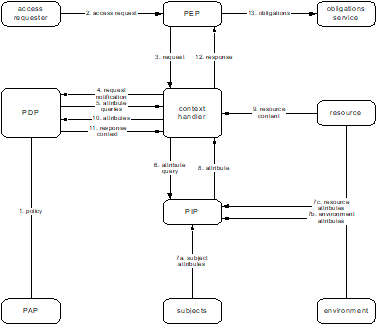
\includegraphics[width=3.94in,height=3.39in]{./media/image67.png}
		\caption{XACML data flow diagram [Source:  eXtensible Access Control Markup Language (XACML) Version 3.0 ]}
		\label{fig:xacml}
	\end{Center}
\end{figure}


%%%%%%%%%%%%%%%%%%%% Figure/Image No: 52 Ends here %%%%%%%%%%%%%%%%%%%%

In general, attributes can describe anything or anyone. Nevertheless, they can be divided into four major categories:

\begin{itemize}
	\item Subject attributes,\\
describing the user by e.g. their age, role, or clearance;

	\item Action attributes,\\
describing the intended action (e.g. read, write, or delete);

	\item Resource (or object) attributes,\\
describing the resource itself (e.g. object type, location, or classification);

	\item Context (or environment) attributes,\\
addressing time, location, or other dynamic aspects.
\end{itemize}

In the IDS, access control is a resource-centric regulation of access requests from subjects (i.e., IDS participants) to resources (i.e., Data Services). Data Owners define attribute-based access control policies for their endpoints. In addition, they define the attribute values a subject must attest in order to grant access to the resource. These attributes may include: 



\begin{itemize}
	\item Specific identity of Connector(s) (only access requests from one or more specific Connectors will be granted);

	\item Connector attributes (only access requests from a Connector that possesses specific attributes will be granted);

	\item Security profile requirements (only access requests from a Connector that meets specific security requirements will be granted; e.g., having a TPM >= 1.2 and doing application isolation).
\end{itemize}

The actual access control decision has to be made within the Connector and can be implemented using technologies such as XACML or JAAS, depending on the implementation of the Connector. The IDS Security Architecture does not dictate a specific access control enforcement language or implementation.

\paragraph{Data Usage Control\\}
%\addcontentsline{toc}{paragraph}{Data Usage Control}

Alongside with data \textit{access} control, regulating access to specific digital resources (e.g., a service or a file), the IDS Security Architecture also supports data \textit{usage} control. In general, the overall goal is to enforce data usage restrictions on the Data Consumer side after access to data has been granted. 

Usage control is an extension of access control (see \textbf{Fehler! Verweisquelle konnte nicht gefunden werden.}). It is about the specification and enforcement of restrictions regulating what may be done with a data asset, and what not. Thus, usage control is concerned with requirements that pertain to data processing (obligations) rather than data access (provisions). Usage control is relevant in the context of intellectual property protection, regulatory compliance, and digital rights management.



%%%%%%%%%%%%%%%%%%%% Figure/Image No: 53 starts here %%%%%%%%%%%%%%%%%%%%

\begin{figure}[H]
	\begin{Center}
		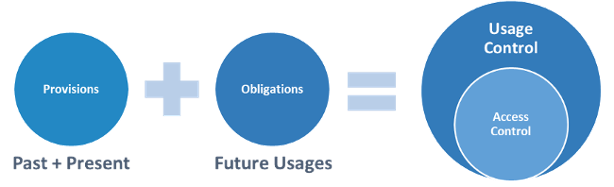
\includegraphics[width=5.68in,height=1.73in]{./media/image68.png}
		\caption{ Data usage control – an extension of data access control}
		\label{fig:_Data_usage_control__an_extension_of_data_access_control}
	\end{Center}
\end{figure}


%%%%%%%%%%%%%%%%%%%% Figure/Image No: 53 Ends here %%%%%%%%%%%%%%%%%%%%

Data usage control in the IDS basically works by attaching data usage policy information to data being exchanged and continuously controlling the way data is processed, aggregated, or forwarded to other endpoints. This data-centric perspective allows Data Providers to continuously control \textit{data flows}, rather than \textit{accesses to services}. At configuration time, data usage policies support developers and administrators in setting up correct data flows.

At runtime, data usage control enforcement prevents IDS Connectors from handling data in an undesired way (for example, by forwarding personal data to public endpoints). Thus, data usage control is both a tool for system integrators to ensure they are not building an architecture that violates security requirements, and an audit mechanism providing evidence of compliant data usage.

The following examples illustrate security requirements that cannot be achieved by data access control, but require data-centric usage control:

\begin{itemize}
	\item \textbf{\textcolor[HTML]{4F81BD}{Secrecy}}\\
Classified data must not be forwarded to nodes which do not have the respective clearance.

	\item \textbf{\textcolor[HTML]{4F81BD}{Integrity}}\\
Critical data must not be modified by untrusted nodes, as otherwise its integrity cannot be guaranteed anymore.

	\item \textbf{\textcolor[HTML]{4F81BD}{Time to live\\
}}Data must be deleted from storage after a certain period of time.

	\item \textbf{\textcolor[HTML]{4F81BD}{Anonymization by data aggregation}}\\
Personal data may be used only in an aggregated form by untrusted parties. To do so, a sufficient number of distinct data records must be aggregated in order to prevent deanonymization of individual records.

	\item \textbf{\textcolor[HTML]{4F81BD}{Anonymization by data substitution}}\\
Data allowing personal identification (e.g., faces in video files) must be replaced by an adequate substitute (e.g., pixelized) in order to guarantee that individuals cannot be deanonymized.

	\item \textbf{\textcolor[HTML]{4F81BD}{Separation of duty}}\\
Two datasets from competitive entities (e.g., two automotive OEMs) must never be aggregated or processed by the same service.

	\item \textbf{\textcolor[HTML]{4F81BD}{Usage scope}}\\
Data may only serve as input for data pipes within the Connector; it must never leave the Connector and be sent to an external endpoint.
\end{itemize}

It is important to note that the purpose of data usage control is to allow the specification of such constraints and enforcing them in the respective system. A precondition of data usage control is that the enforcement mechanism itself is trusted; i.e., data usage control itself does not establish trust in an endpoint, but rather builds upon an existing trust relationship and facilitates enforcement of legal or technical requirements, such as service level agreements (SLAs) or data privacy regulations. Thus, users must be aware that data usage control will only provide certain enforcement guarantees if applied on highly trusted platforms, such as Trusted Connectors in the International Data Spaces (see Section 3.2).


\subparagraph*{Technical enforcement, organizational rules, and legal contracts\\}
%\addcontentsline{toc}{subparagraph}{Technical enforcement, organizational rules, and legal contracts}
Data usage control can be implemented by means of a machine-readable contract, which is expected to be fulfilled by a party. It is a way to track and trace data as it is used within different systems and to collect evidence of the violation of agreed usage constraints. With that in mind, solutions range from organizational rules or legal contracts to completely technical ways of enforcing usage restrictions. For example, an organizational rule (e.g. a company policy) could state that employees must not use removable storage devices, such as USB sticks. Similarly, a technical form of enforcement, such as group policies specified by the Windows operating system, can prevent employees from using removable storage devices. In some scenarios, organizational rules, legal contracts, and technical rules can be used interchangeably. In other scenarios, the three forms can be used to complement each other. In the long run, it can be expected that organizational rules and legal contracts will increasingly be replaced by technical forms of enforcement (as illustrated in Figure 413).



%%%%%%%%%%%%%%%%%%%% Figure/Image No: 54 starts here %%%%%%%%%%%%%%%%%%%%

\begin{figure}[H]
	\begin{Center}
		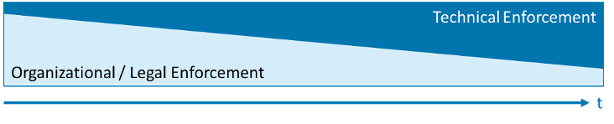
\includegraphics[width=5.33in,height=1.08in]{./media/image69.png}
		\caption{ Technical enforcement vs. organizational/legal enforcement}
		\label{fig:_Technical_enforcement_vs_organizationallegal_enforcement}
	\end{Center}
\end{figure}


%%%%%%%%%%%%%%%%%%%% Figure/Image No: 54 Ends here %%%%%%%%%%%%%%%%%%%%


Enforcement of data usage restrictions can be characterized and implemented in different forms. Organizational rules or legal contracts can be substituted, or at least accompanied, by technical solutions, which introduce a new level of security. Vice versa, technical solutions can be accompanied by organizational rules or legal contracts (e.g., to compensate missing capabilities of the technical solution).

Although it is a commonly used solution to address data usage control restrictions by organizational rules, the IDS-RAM focuses on technical enforcement.

\subparagraph*{ Enforcement\\}
%\addcontentsline{toc}{subparagraph}{ Enforcement}
To enforce data usage restrictions, a system’s actions need to be monitored and potentially intercepted by control points (i.e., Policy Enforcement Points, PEPs). These actions must be judged by a decision engine (i.e., a Policy Decision Point, PDP) for requesting permission or denial. In addition to just allowing or denying an action, the decision engine may also require modification of the action. A PEP component encapsulates the enforcement.


\textbf{Decision and Information\\}


Enforcement relies on a decision. The PDP has the responsibility to answer incoming requests (e.g., system actions) from a PEP in the form of a decision (see  Figure 414 ). Decision-making based on usage restriction is also called (policy) evaluation. There are several types of evaluation, such as event-based or flow-based approaches.



%%%%%%%%%%%%%%%%%%%% Figure/Image No: 55 starts here %%%%%%%%%%%%%%%%%%%%

\begin{figure}[H]
	\begin{Center}
		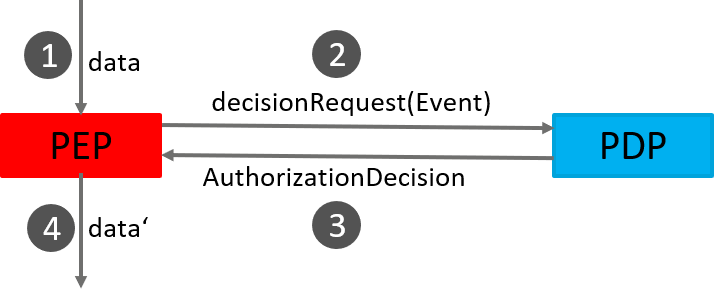
\includegraphics[width=3.33in,height=1.94in]{./media/image70.png}
		\caption{Communication Policy Enforcement Point and Policy Decision Point}
		\label{fig:Communication_Policy_Enforcement_Point_and_Policy_Decision Point}
	\end{Center}
\end{figure}


%%%%%%%%%%%%%%%%%%%% Figure/Image No: 55 Ends here %%%%%%%%%%%%%%%%%%%%
\par


For event-based systems, data usage transactions are represented as events including attributes to characterize the data usage. Event processing can be differentiated into simple processing (e.g., event-condition-action paradigm) and stream processing (e.g., sliding window) of events. The terms $"$ event stream processing$"$  and $``$complex event processing$"$  are often used interchangeably.

For example: It is possible to model the transition of data as an event with attributes about the data itself and the recipient. The attributes contain metadata and information on the target system (e.g., supplier management system). The decision engine makes a deny decision if the target system does not correspond to the expected supplier management system.

The policy decision may also depend on additional information that is not present in the intercepted system action itself. This includes information about the context, such as data flows or the geographical location of an entity. It is also possible to specify pre- or post-conditions that have to hold before (e.g., integrity check of the environment) and after (e.g., data item is deleted after usage) decision-making. In addition, it is possible to define on-conditions that have to hold during usage (e.g., only during business hours). These conditions usually specify constraints and permissions that have to be fulfilled before, during, and after using data (see  Figure 415   ). 



%%%%%%%%%%%%%%%%%%%% Figure/Image No: 56 starts here %%%%%%%%%%%%%%%%%%%%

\begin{figure}[H]
	\begin{Center}
		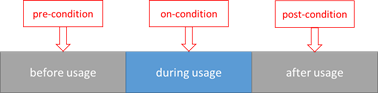
\includegraphics[width=3.94in,height=0.97in]{./media/image71.png}
		\caption{Usage Control Pre-, On-, and Post-Conditions}
		\label{fig:Usage_Control_Pre-_On-_and Post-Conditions}
	\end{Center}
\end{figure}


%%%%%%%%%%%%%%%%%%%% Figure/Image No: 56 Ends here %%%%%%%%%%%%%%%%%%%%


A Policy Information Point (PIP) provides missing information for decision-making. In addition, such a component can be used to get contextual information for or about the system action intercepted (e.g., data flow information, geolocation of the requesting device).

\textbf{Specification, Management, and Negotiation}\\


Another important aspect of data usage control is the specification and management of usage restrictions. Data Providers have to express data usage restrictions in a more or less formal way. For technical enforcement, the specification must produce a machine-readable output. The Policy Administration Point (PAP) is the entry point for specification of usage policies, often via a user-friendly graphical interface.

A Policy Management Point (PMP) is responsible for the management of usage policies. Hence, the component is concerned with the policy’s lifecycle. This includes instantiation, negotiation, deployment, and revocation of usage restrictions, as well as conflict detection and resolution.

There are two ways to make usage restriction information available: 

\begin{itemize}
	\item Usage restriction policy information can be attached to the data that is about to be exchanged. This type of policy is called sticky policy\footnote{ M. C. Mont and S. Pearson, "Sticky Policies: An Approach for Managing Privacy across Multiple Parties," Computer, pp. 60-68, 09 September 2011.  }. Following this approach, data is encrypted before it is sent to a Data Consumer, and it can only be decrypted if the Data Consumer fully and explicitly accepts the usage restrictions specified. 

	\item A usage restriction policy can be stored independently of the data it relates to (for instance, in a central component, such as a PMP/PRP). In this case, the management component has the responsibility to exchange usage restriction information between different systems.
\end{itemize}

The management of usage policies becomes especially important when data is to be exchanged across system boundaries. Every time data crosses system boundaries, the target system must be prepared for the protection of incoming data (i.e. it has to deploy the corresponding policy). 

Policy negotiation is also part of policy management. As enforcement mechanisms can work differently across different systems or technologies, abstract policies may have different instantiations. Hence, usage policies must always be instantiated on the target system.

\subparagraph*{Usage Control Building Blocks \\}
%\addcontentsline{toc}{subparagraph}{Usage Control Building Blocks }
 This section outlines which components the  International  Data Spaces uses to integrate data usage control technologies. The first subsection deals with the IDS Information Model and its modules addressing data usage control. The subsequent sections are about the Trusted Connector and the Apache Camel interceptor.  


\textbf{Information Model}\\
IDS  Information Model is a modular vocabulary describing the capabilities of IDS infrastructure components, such as the Connector or the Data Endpoints. Descriptions of data provided by Data Endpoints are published at dedicated Broker registries, allowing potential Data Consumers to search for and identify data that is relevant (semantics) and applicable (quality) for their particular  purpose, and to assess in advance data’s affordability (price) and usability (restrictions).

Extending the Open Digital Rights Language (ODRL)\footnote{ R. Iannella, S. Guth, D. Paehler and A. Kasten, "ODRL Version 2.1 Core Model," 05 03 2015. [Online]. Available: https://www.w3.org/community/odrl/model/2.1/.}  , a W3C standard, the Information Model’s Usage Control module provides machine-readable specifications of usage control policies (see section 3.4.4.1.1). These specify actions that a party is prohibited or permitted to do with regard to given a data asset. In addition, they codify any potentially involved duties. Despite a simple core model, which is depicted in  Figure 416 , ODRL policies are a formal way to declaratively express usage contracts at a specification level. This way, the Information Model provides a technology-agnostic, consistent representation of usage control policies across the International Data Spaces. 



%%%%%%%%%%%%%%%%%%%% Figure/Image No: 57 starts here %%%%%%%%%%%%%%%%%%%%

\begin{figure}[H]
	\begin{Center}
		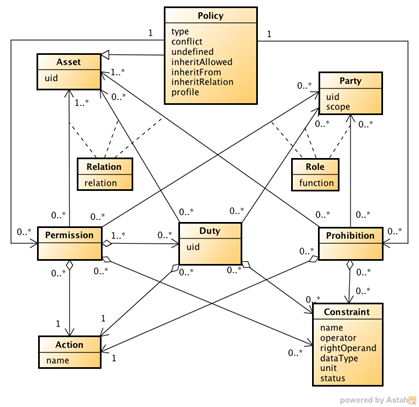
\includegraphics[width=4.36in,height=4.24in]{./media/image72.png}
		\caption{ODRL Core Model 2.1 (ODRL Version 2.1 Common Vocabulary Final Specification: 5 March 2015)}
		\label{fig:odrl}
	\end{Center}
\end{figure}


%%%%%%%%%%%%%%%%%%%% Figure/Image No: 57 Ends here %%%%%%%%%%%%%%%%%%%%

In order to implement and enforce usage policies at a specification level within individual target environments, it is necessary to map organizational and technical measures to the individual target environments. While organizational measures are out of scope here, technical measures involve a variety of additional information sources (PIPs) and tight integration with the host environment (PEPs). Here, the Information Model enhances ODRL constructs via predefined extension $``$hooks$"$  to support mapping onto lower-level, implementation-oriented policy languages (e.g., IND²UCE XML).


For example, the ODRL Constraint class expresses logical conditions that govern the applicability of a Rule. Here, an Operator (eq) relates the Left Operand (a predicate like absolutePosition) to a Right Operand (dynamic or predefined value). On the one side, the Information Model extends the group of predefined predicates\footnote{ R. Iannella, M. Steidl, S. Myles and V. Rodríguez-Doncel, "ODRL Vocabulary $\&$  Expression - 3.14.9 Left Operand," 26 09 2017. [Online]. Available: https://www.w3.org/TR/odrl-vocab/$\#$ term-LeftOperand.  } in order to support decision-making in particular scenarios of the IDS, such as data residency\footnote{ The Object Management Group, "Data Residency Working Group," [Online]. Available: http://www.omg.org/data-residency/.  }; on the other side, it defines a configuration overlay (b) to tie the abstract predicates (a) to an operable programming logic supplied by the respective target environment (c), as illustrated by Figure 417.



%%%%%%%%%%%%%%%%%%%% Figure/Image No: 58 starts here %%%%%%%%%%%%%%%%%%%%

\begin{figure}[H]
	\begin{Center}
		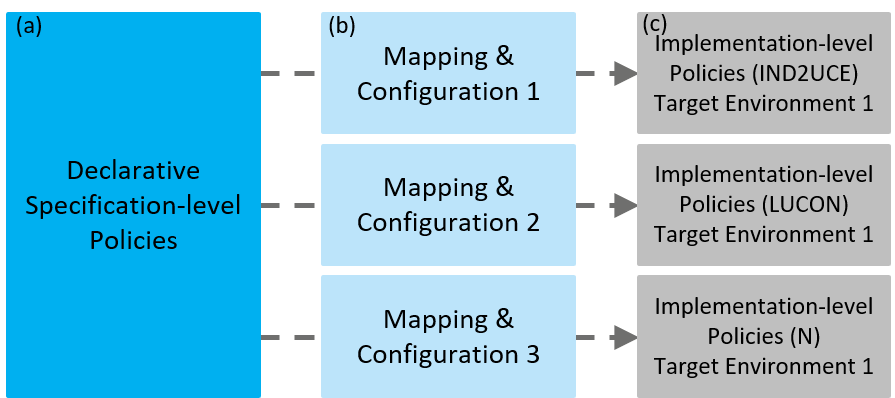
\includegraphics[width=4.94in,height=2.17in]{./media/image73.png}
		\caption{Examples of mapping among policy language levels}
		\label{fig:Examples_of_mapping_among_policy_language_levels}
	\end{Center}
\end{figure}


%%%%%%%%%%%%%%%%%%%% Figure/Image No: 58 Ends here %%%%%%%%%%%%%%%%%%%%

\textbf{Trusted Connector\\}

Usage control only makes sense in an ecosystem where a certain level of trust can be established and maintained for all participants. To enable the establishment of trusted relationships, the central technological components used for data processing and data exchange need to be trustworthy. The IDS Connector is the central component for data exchange and data processing in the International  Data Spaces, and thus a central component that needs to be trusted.

The IDS Connector (see previous sections) focuses on security and delivers a trusted platform, incorporating crucial building blocks:

\begin{itemize}
	\item identity $\&$  trust management for authenticating communicating parties (e.g., other Connectors) and shaping trusted relationships between partners;

	\item a trusted platform as a baseline for secure data processing;

	\item trustworthy communication based on authenticated and encrypted connections; and

	\item access $\&$  usage control.
\end{itemize}

Instances of the Trusted Connector enable remote integrity verification, so the integrity of the deployed software stack can be guaranteed before granting access to data.

The Trusted Connector guarantees a controlled execution environment for data services and supports the creation of trusted relationships. A general constraint is one that remains for all deployed IT systems: As long as physical or logical access is granted to administrators, protection against data theft by malicious partners is almost impossible to prevent. The International Data Spaces is seen as a network of partners that are provided with the technical means to fulfill their obligations and support in deciding what partners to trust and to define reasonable access conditions.


\textbf{Apache Camel interceptor (example)\\}

An IDS Connector may use Apache Camel to coordinate the data flow between different systems and applications. From a technical point of view, the developer does this by using pipelining, which is a dominant paradigm of Apache Camel for connecting different nodes in a route definition. The basic idea of a pipeline is that Apache Camel uses the output of one node as input to the next node. Every node in such a route is a processor, except for the initial endpoint (as shown in  Figure 418 ). 



%%%%%%%%%%%%%%%%%%%% Figure/Image No: 59 starts here %%%%%%%%%%%%%%%%%%%%

\begin{figure}[H]
	\begin{Center}
		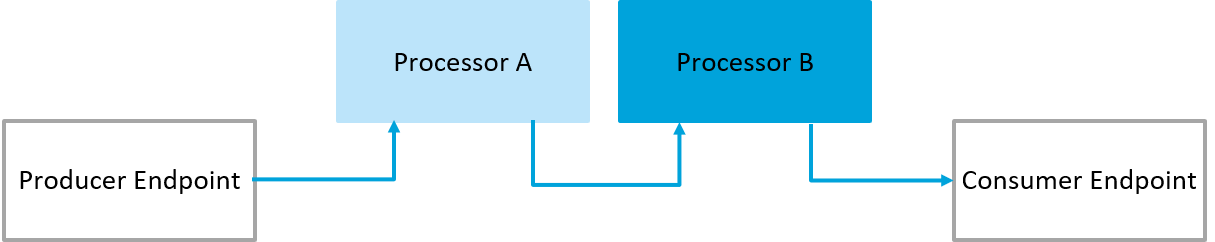
\includegraphics[width=3.94in,height=0.81in]{./media/image74.png}
		\caption{Apache Camel pipeline (example)}
		\label{fig:Apache_Camel_pipeline}
	\end{Center}
\end{figure}


%%%%%%%%%%%%%%%%%%%% Figure/Image No: 59 Ends here %%%%%%%%%%%%%%%%%%%%

In order to control the usage of data, one approach can be to intercept the data flow between the services and applications. Figure 419 shows as example of how developers can do this. Apache Camel offers the possibility to integrate interceptors that it executes every time before and after a processor is working.



%%%%%%%%%%%%%%%%%%%% Figure/Image No: 60 starts here %%%%%%%%%%%%%%%%%%%%

\begin{figure}[H]
	\begin{Center}
		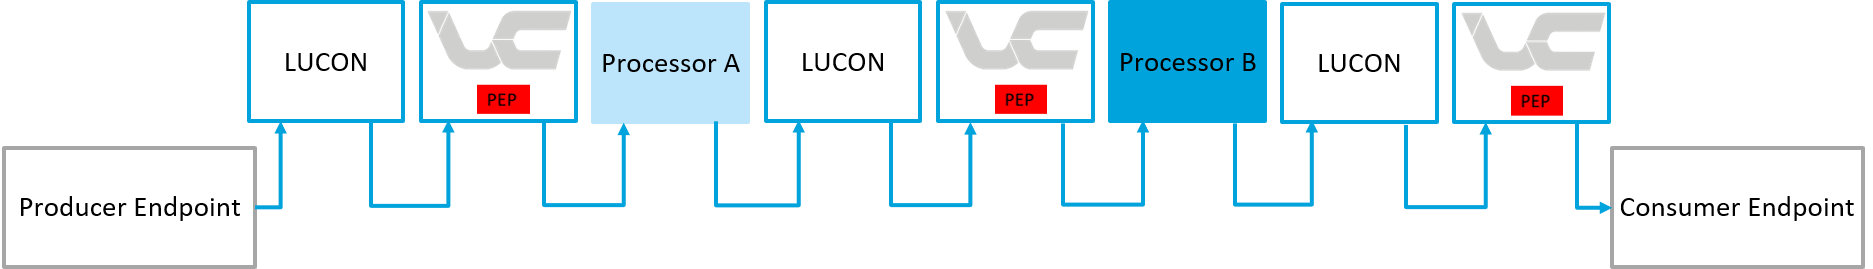
\includegraphics[width=5.11in,height=0.74in]{./media/image75.png}
		\caption{Intercepting Apache Camel data flows}
		\label{fig:Intercepting_Apache_Camel_data_flows}
	\end{Center}
\end{figure}


%%%%%%%%%%%%%%%%%%%% Figure/Image No: 60 Ends here %%%%%%%%%%%%%%%%%%%%


As the International Data Spaces provides an Information Model (see Section 3.1),
% ToDo: should refer to section 3.4
additional metadata enhances the data transferred via the route, thereby enabling better usage control enforcement. The Connector attaches the metadata to the data package, as explained in section 3.4. In addition, a PIP is able to resolve more metadata during the decision-making process if necessary.

This paradigm also works across company borders, as data always flows through the IDS Connector and the Apache Camel interceptor, respectively (as shown in Figure 420 ). When reaching the receiving Connector, the respective policy to protect the data is automatically instantiated.


%%%%%%%%%%%%%%%%%%%% Figure/Image  starts here %%%%%%%%%%%%%%%%%%%%

\begin{figure}[H]
	\begin{Center}
		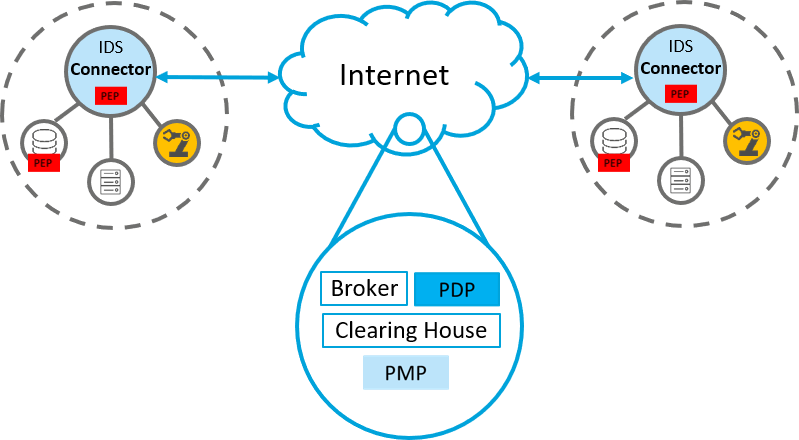
\includegraphics{./media/image76.png} %[width=5.11in,height=0.74in]
		\caption{Data flow across company borders}
		\label{fig:Data_flow_across_company_borders}
	\end{Center}
\end{figure}


%%%%%%%%%%%%%%%%%%%% Figure/Image Ends here %%%%%%%%%%%%%%%%%%%%


Depending on the policies available, this way of enforcement is not enough to cover all possible use cases and full usage control. 

\subparagraph*{Roles Involved in Usage Control\\}
%\addcontentsline{toc}{subparagraph}{Roles Involved in Usage Control}
Usage control is a cross-sectional concept and technology, which involves several IDS Roles.

\textbf{Broker}\\
The IDS Broker manages connector self-descriptions that can contain Usage Policies. Therefore the Broker must be able to support Usage Policies. In addition the connector self-description itself may be subject of Usage Policies. 

\textbf{Connector}\\
The Connector is the main technical component for implementing usage control. Hence, usage control enhanced Connectors, such as the Trusted Connector, contain relevant components to perform usage control enforcement as Data Consumer (PEPs, such as the Apache Camel interceptor; PDPs, PMPs). However, PMPs and PDPs need not be part of the Connector. In addition, Connectors as Data Providers should provide the technology-dependent policies to the data they provide – for all kinds of systems and enforcement technologies that are part of the ecosystem.

\textbf{Clearing House}\\
By means of Data Provenance Tracking (as described in the next section), it is possible to track the usage of data and the enforcement of usage restrictions. The Clearing House is able to use this data later on.

\textbf{App Store}\\
Data Apps can take advantage of usage control technology. The IDS App Store needs to be able to provide information as to whether a Data App implements such technology.

\textbf{App Provider}\\
For Data Apps to take advantage of usage control technology, App Providers need to implement certain components, such as control points (i.e., PEPs), into their application.


\paragraph*{Data Provenance Tracking\\}
%\addcontentsline{toc}{paragraph}{Data Provenance Tracking}
Data provenance tracking is closely related, but also complementary to distributed data usage control. It has its origins in the domain of scientific computing, where it was introduced to trace the lineage of data. Data provenance tracking thereby allows finding out when, how and by whom data was modified, and which other data influenced the process of creating new data items.

This kind of traceability is similar to the data protection requirements a data controller is confronted with, so as to be able to fulfill its data subjects’ right to access. It is also closely related to the question of proving compliance with contracts, agreements, or legal regulations. And data provenance tracking can be used to facilitate clearing in decentralized data ecosystems, since it is capable of aggregating information concerning data exchange transactions and data usage.

However, while distributed data usage control is concerned with the enforcement of rights and duties when exchanging data across system boundaries, the focus of data provenance tracking is on transparency and accountability. In other words: While a Policy Enforcement Point (PEP) serving for distributed data usage control in most cases needs to be able to proactively intercept data usage actions within the control flow (i.e. preventive enforcement), a PEP for data provenance tracking only needs to passively observe, interpret and log data exchange transactions and data usage for retrospective examination (in terms of usage control, this kind of enforcement is denoted as $``$detective enforcement$"$ ). Despite this fact, a data provenance tracking infrastructure can be built upon the same PEPs as distributed data usage control. Furthermore, data provenance tracking does not require a policy specification language, but rather a specification of how observed actions are to be interpreted in terms of data flow or data usage (i.e., a so-called data flow semantics specification). By this, data provenance tracking maintains a data flow model that keeps track of the particular representations of data items. This kind of information can also be leveraged for data usage control enforcement; i.e., the data flow model is implemented as a Policy Information Point (PIP).


\subparagraph*{Operating Principle \\}
%\addcontentsline{toc}{subparagraph}{Operating Principle }
The operating principle of data provenance tracking is very similar to the operating principle of distributed data usage control. Data provenance tracking relies on passive monitoring technology (e.g., PEPs), which deliver events indicating data usage or data flows for being logged. For this, a PEP needs to convey a semantic description of the data usage or data flows its events indicate. The data provenance tracking infrastructure provides a data flow tracking component, which understands such semantics specifications. The PEP also needs to forward events together with metadata (including a unique identifier of the data’s content), so that logged transactions can be attributed to data content when data provenance is aggregated or queried.


\subparagraph*{Architecture\\}
%\addcontentsline{toc}{subparagraph}{Architecture}
The PEP resides within the message routing component of the  Connector (or Data App). It is registered at the data flow tracking component via a registry component (i.e., a local Policy Management Point, PMP). The same applies for the data flow tracking component. Thereby a PEP can query the local PMP for the communication interface of the local data flow tracking component, which is then used to deploy semantics specifications for its observed events and to forward actual events during operation.



%%%%%%%%%%%%%%%%%%%% Figure/Image No: 61 starts here %%%%%%%%%%%%%%%%%%%%

\begin{figure}[H]
	\begin{Center}
		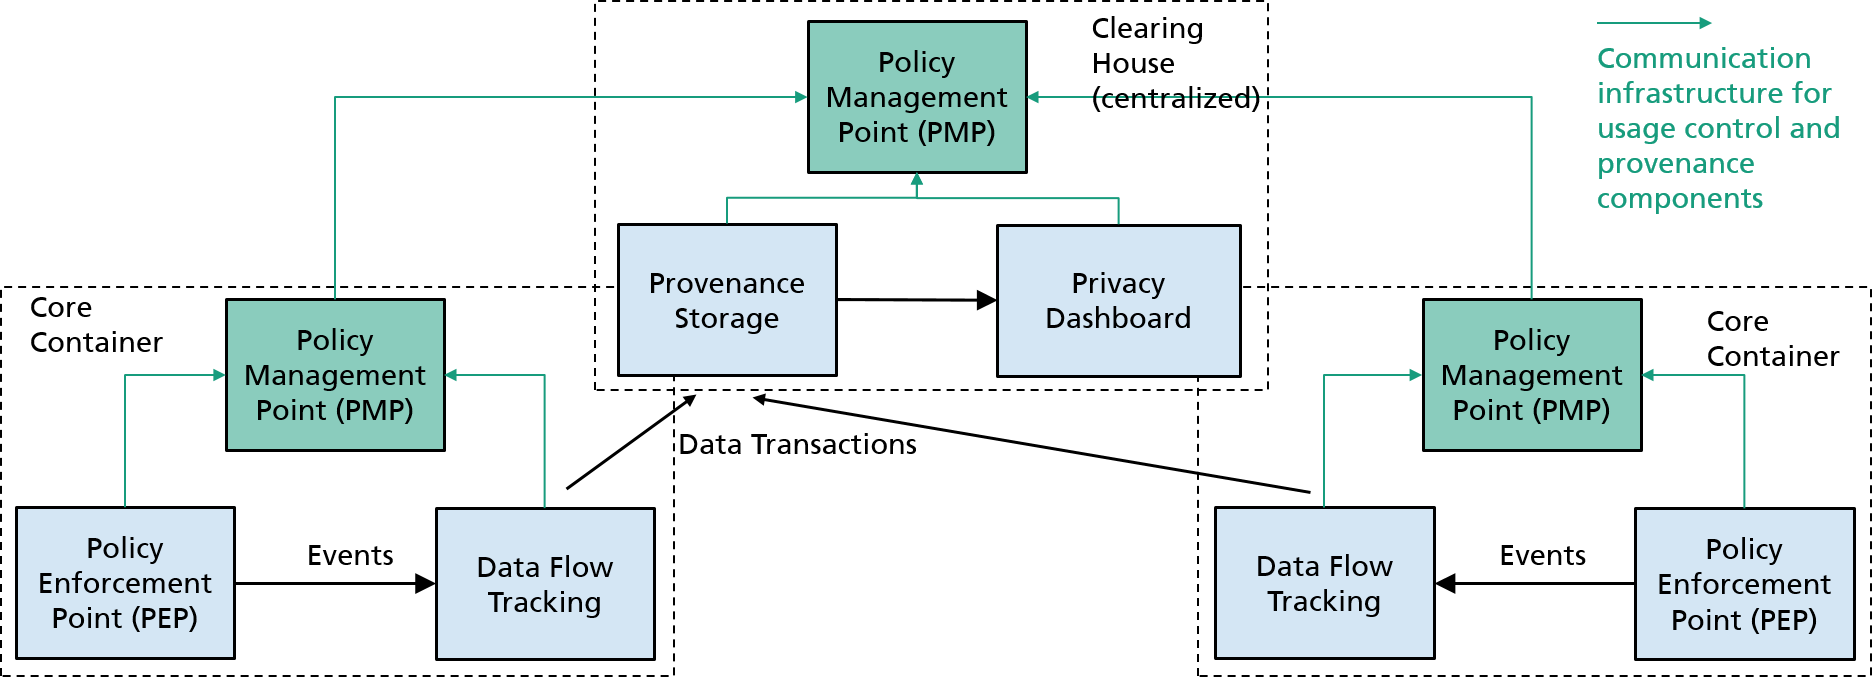
\includegraphics[width=6.53in,height=2.36in]{./media/image77.png}
		\caption{Architecture with centralized  component for provenance information storage}
		\label{fig:centralized_provenance}
	\end{Center}
\end{figure}


%%%%%%%%%%%%%%%%%%%% Figure/Image No: 61 Ends here %%%%%%%%%%%%%%%%%%%%



%%%%%%%%%%%%%%%%%%%% Figure/Image No: 62 starts here %%%%%%%%%%%%%%%%%%%%

\begin{figure}[H]
	\begin{Center}
		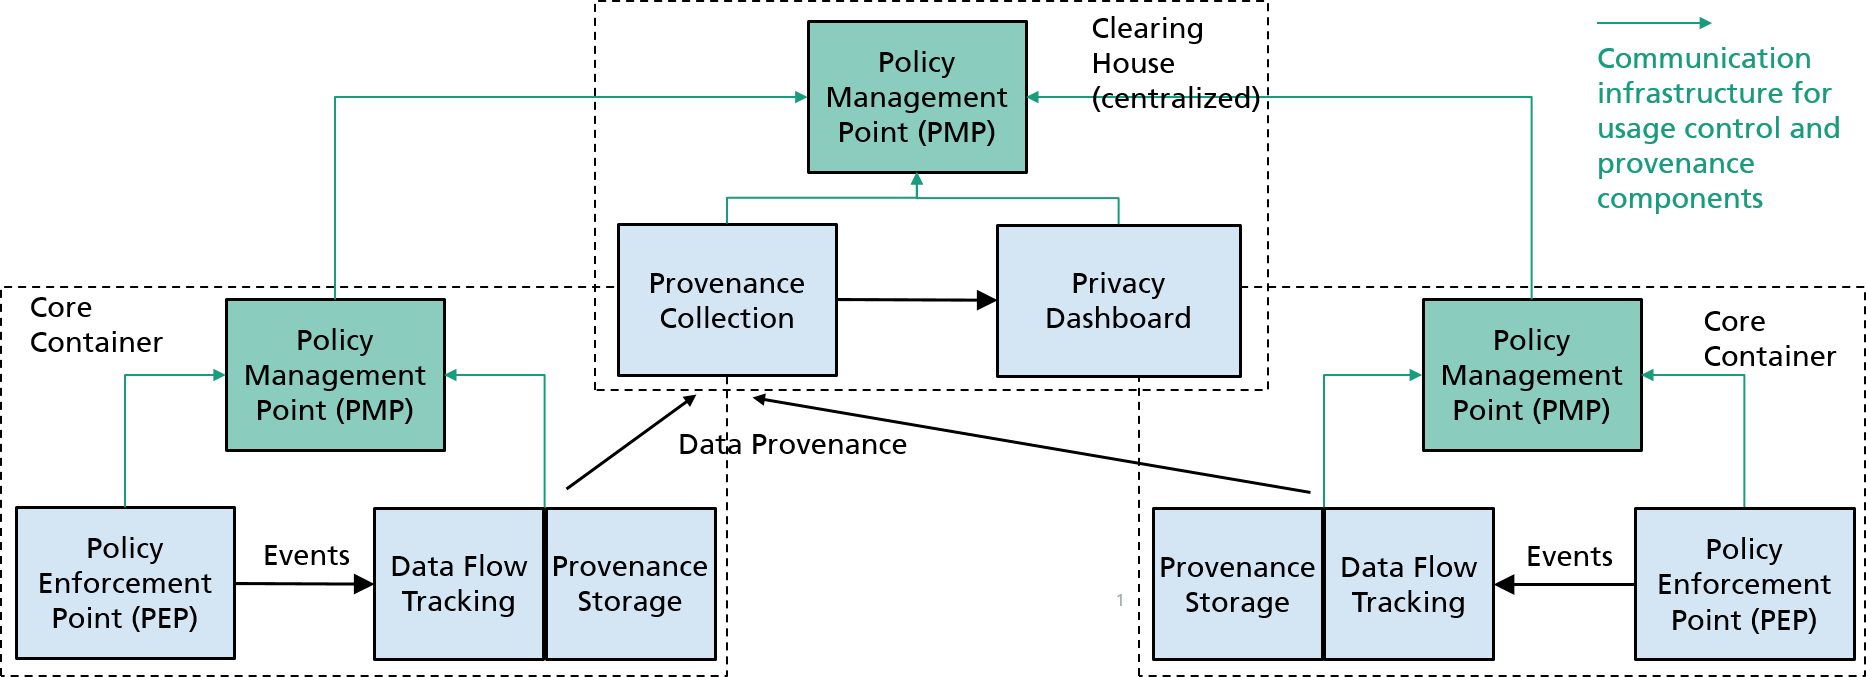
\includegraphics[width=6.53in,height=2.37in]{./media/image78.png}
		\caption{Architecture with distributed component for provenance information storage}
		\label{fig:distributed_provenance_tracking}
	\end{Center}
\end{figure}


%%%%%%%%%%%%%%%%%%%% Figure/Image No: 62 Ends here %%%%%%%%%%%%%%%%%%%%

Data provenance information is queried at a Privacy Dashboard, which is accessible via a Clearing House. The Privacy Dashboard returns a provenance graph for the unique identifier of data content. There are two options for storing data provenance information:


\begin{itemize}
	\item Centralized architecture (see Figure \ref{fig:centralized_provenance}): A Provenance Storage Point (ProSP) is attached to the Clearing House. After data usage or a data flow has been observed by the data flow tracking component inside the Connector, the transaction is logged at this ProSP.

	\item Distributed architecture (see Figure \ref{fig:distributed_provenance_tracking}): Each Connector is equipped with a ProSP, which is directly connected to the data flow tracking component. The Clearing House accommodates only a stateless Provenance Collection Point (ProCP), which aggregates provenance information coming in from the distributed ProSPs whenever a query occurs at the Privacy Dashboard.
\end{itemize}


\subparagraph*{Communication\\}
%\addcontentsline{toc}{subparagraph}{Communication}
The local data flow tracking component inside the  Connector has to be able to communicate with the centralized data provenance infrastructure (i.e., ProSP or ProCP). For this, a so-called Root-PMP is attached to the Clearing House. Here, the central components register their communication interfaces, and so do the local PMPs of the Connectors. Using these interfaces, provenance information is passed on to the central ProSP/ProCP.

Analogous to this hierarchical communication infrastructure, the provenance information of each unit of data content is a tree, a so-called provenance graph. It is either maintained at a central ProSP or at the distributed ProSPs located inside the Connectors. In the latter case, a centralized ProCP at the Clearing House aggregates the various sub-trees for a unique data content identifier from distributed ProSPs (i.e. it consolidates the provenance information by merging the subtrees).


\subparagraph*{Integration with Distributed Usage Control\\}
%\addcontentsline{toc}{subparagraph}{Integration with Distributed Usage Control}
In complex usage control scenarios, such as establishing data sovereignty for managing globally distributed supply chains, data is passed on from one Data Consumer to another. Depending on the usage control policy in place, data may be forwarded in its original form, or it may be somehow processed, aggregated, or anonymized before being forwarded. This indicates the relevance of establishing transparency concerning data flows and data usage in compliance with usage control policies, business contracts, or legal regulations. For this purpose, distributed data usage control and data provenance tracking complement each other. As explained before, the PEPs used for usage control (detective enforcement) can also serve as a basis for data provenance tracking, whereas in turn data provenance information can be fed back into usage control enforcement (i.e., a usage control PDP can query for all locations of representations of some given data content protected by a usage control policy).

Further synergies can be exploited by employing the same communication infrastructure for distributed data usage control and data provenance tracking. The hierarchical PMP structure (as described in the previous section) can also enable usage control components to interact across different IDS Connectors (e.g., for shipping policies to other Connectors, deploying and revoking policies, etc.).

\subparagraph*{Data Provenance Tracking Addressed by the Different Layers of the IDS-RAM\\}
%\addcontentsline{toc}{subparagraph}{Data Provenance Tracking Addressed by the Different Layers of the IDS-RAM}
\textbf{Business Layer}\\
Data provenance tracking primarily supports the work of the Clearing House. It provides the means to establish a centralized audit log aggregating tracking information concerning data exchange transactions and data usage.

\textbf{Functional Layer}\\
Data provenance tracking does not directly affect the core functionality of the IDS, since it is typically implemented on top of a usage control infrastructure, or based on passive monitoring technology. However, data provenance tracking may enhance the functionality of the IDS by offering functions for clearing and accounting, provided tracking is sufficiently accurate (e.g., in terms of delivering concrete numbers of data users or a concrete duration of data use). Data Apps might also be considered as content/data the usage of which can be tracked by data provenance technology.

\textbf{Process Layer}\\
Data provenance tracking is integrated in the $``$Exchange Data$"$  process (or, to be more precise, in the $``$Query Data$"$  sub-process). Data provenance tracking components in the Connector of the Data Provider as well as in the Connector of the Data Consumer signal to the data provenance storage component at the Clearing House that data has been successfully sent or received, respectively. This signaling is implemented based on events intercepted by PEPs for distributed data usage control.

\textbf{Information Laye}\\
Data provenance tracking can be orchestrated for different purposes. Regarding the IDS, the most important goals are establishing transparency and being able to prove compliance to contracts, agreements, or legal regulations. Reliability of content is a secondary goal of data provenance tracking in the IDS. While making the lineage of data traceable is the original purpose of data provenance tracking, this requires either specific, data provenance enabled Data Apps or the use of dedicated PEPs for these Data Apps.


\textbf{System Layer}\\
Reliability of data provenance information strongly depends on trustworthy Connectors and Data Apps (including their PEPs). It is recommended to integrate data provenance tracking into Trusted Connectors and to certify Data Apps that are enabled for data provenance tracking and data usage control.
